\documentclass[../basicOrbitalDynamics.tex]{subfiles}
\graphicspath{{\subfix{../images/}}}
\begin{document}

With the geometry of an entire orbit known, physical quantities can be determined.

\bigskip\bigskip
\subsection{Angular Momentum}\label{sec:Angular Momentum Geometric}

The angular momentum $h$ of a satellite is, as was proven earlier, conserved. From the physical definition of angular momentum ($\vv{h}=\vv{r}\times\vv{v}$), the following can be observed:
\begin{equation}\label{Angular Momentum Physical Definition}
    h=rv_\perp
\end{equation}

Equation \eqref{SLR h and mu}, which describes the semi-latus rectum from physical parameters, can be set equal to \eqref{SLR a and e}, which describes the semi-latus rectum from geometric definitions. This will allow for the angular momentum to be isolated.
\begin{align*}
    \frac{h^2}{\mu} & = a(1-e^2)           \\
    h^2             & = a(1-e^2)\mu        \\
    h               & = \sqrt{a\mu(1-e^2)} \\
\end{align*}

This equation is not defined for parabolic orbits. Note that in a hyperbolic orbit, the signs of $a$ and $1-e^2$ are both negative, so the square root is still real.
\begin{equation}\label{Angular Momentum Geometric Definition}
    h=\sqrt{a\mu(1-e^2)}
\end{equation}


\bigskip\bigskip
\subsection{Period}\label{Sec:Period Geometric}

The area of a closed ellipse is known from geometry.
\[\text{Area}=\pi{}ab\]

From Kepler's first law (which was proven in Section \ref{sec:Kepler's First Law}), an equation exists that tells us the area of an orbit as a function of time (Equation \eqref{Kepler's First Law}). If the entire period $T$ is used as the time step, then the area can be found. Because the period is not defined for a hyperbolic orbit, the semi-minor axis will not use an absolute value. However, it turns out that this omission is inconsequential anywho, as the $\sqrt{1-e^2}$ term will cancel out.
\begin{align*}
    \text{Area}          & = \frac{h}{2}P                                     \\
    \pi{}ab              & = \frac{h}{2}P                                     \\
    \pi{}a^2\sqrt{1-e^2} & = \frac{h}{2}P                                     \\
    \pi{}a^2\sqrt{1-e^2} & = \frac{\sqrt{a\mu(1-e^2)}}{2}P                    \\
    T                    & = \frac{2\pi{}a^2\sqrt{1-e^2}}{\sqrt{a\mu(1-e^2)}} \\
                         & = 2\pi{}a^2\sqrt{\frac{1-e^2}{a\mu(1-e^2)}}        \\
                         & = \sqrt{\frac{4\pi^2a^4}{a\mu}}                    \\
\end{align*}
\begin{equation}\label{Period Geometric}
    T = \sqrt{\frac{4\pi^2a^3}{\mu}}
\end{equation}

Hyperbolic and parabolic orbits do not have periods, as they are not closed.

\bigskip\bigskip
\subsection{Specific Energy}\label{sec:Specific Energy}

Specific energy $\varepsilon$ is the total energy in an orbit, normalized with respect to the mass of the satellite. Total energy is the sum of the kinetic energy and gravitational potential energy (with the potential constant set so that, as distance approaches infinity, the potential function vanishes).
\begin{align*}
    \varepsilon & =\frac{\text{KE}+\text{PE}}{m}                             \\
                & =\frac{1}{m}(\text{KE}+\text{PE})                          \\
                & =\frac{1}{m}\left(\frac{1}{2}mv^2+\frac{-\mu{}m}{r}\right) \\
                & =\frac{v^2}{2}-\frac{\mu{}}{r}                             \\
\end{align*}

Conservation of specific energy was proven earlier, but a more useful expression for it can be found.

Specific energy is constant, so it will be found at periapsis. First, velocity must be found by setting Equation \eqref{Angular Momentum Physical Definition} (the physical definition of angular momentum, $rv_\perp$) equal to its derived counterpart ($\sqrt{a\mu(1-e^2)}$) from Equation \eqref{Angular Momentum Geometric Definition}. Note that at periapsis, velocity is entirely normal to the radial vector, so $v_\perp=v$, and recall that Equation \eqref{Periapsis Radius Geometric} states $\st{r}{pe}=a(1-e)$.
\begin{align*}
    \st{r}{pe}\st{v}{pe} & = \sqrt{\mu{}a(1-e^2)}                       \\
    a(1-e)\st{v}{pe}      & = \sqrt{\mu{}a(1-e)(1+e)}                    \\
    \st{v}{pe}            & = \sqrt{\frac{\mu{}a(1-e)(1+e)}{a^2(1-e)^2}} \\
    \st{v}{pe}            & = \sqrt{\frac{\mu{}(1+e)}{a(1-e)}}           \\
\end{align*}

Now, specific energy can be found.
\begin{align*}
    \varepsilon & = \frac{1}{2}v^2-\frac{\mu}{r}                            \\
                & = \frac{1}{2}\frac{\mu{}(1+e)}{a(1-e)}-\frac{\mu}{a(1-e)} \\
                & = \frac{\mu{}(1+e)}{2a(1-e)}-\frac{2\mu}{2a(1-e)}         \\
                & = \frac{\mu{}(1+e)-2\mu}{2a(1-e)}                         \\
                & = \frac{\mu{}(e-1)}{2a(1-e)}                              \\
                & = \frac{-\mu}{2a}                                         \\
\end{align*}

Note that because $a$ is infinite for a parabola (see \ref{sec:Analysis of parabolic trajectories}), $\varepsilon=0$ for parabolic orbits, Since $a<0$ for hyperbolas, $\varepsilon>0$ in hyperbolic orbits.
\begin{equation}\label{Specific Energy Geometric}
    \varepsilon=\frac{-\mu}{2a}
\end{equation}

This is valid for \textit{all} orbits. Of note is the fact that eccentricity plays no role in specific energy of an orbit, aside from to determine its sign in extreme cases. This has an interesting ramification for orbital dynamics; since a burn normal to the velocity vector and in plane with the orbit performs no work, it must not change the specific energy of the orbit. While other parameters, such as inclination, can change without the specific energy changing, that requires out-of-plane maneuvers. This implies (correctly) that burning normal to the velocity has the effect of changing its eccentricity or inclination but not its semi-major axis.

\bigskip\bigskip
\subsection{Velocity}\label{sec:Velocity}

Specific energy found in Equation  \eqref{Specific Energy Geometric} can be set equal to the physical definition of specific energy, so that $v$ can be solved for.
\begin{align*}
    \frac{1}{2}v^2-\frac{\mu}{r} & =\frac{-\mu}{2a}                     \\
    \frac{1}{2}v^2               & =\frac{\mu}{r}-\frac{\mu}{2a}        \\
    v^2                          & =\frac{2\mu}{r}-\frac{\mu}{a}        \\
    v                            & =\sqrt{\frac{2\mu}{r}-\frac{\mu}{a}} \\
\end{align*}

The $\frac{-\mu}{a}$ term vanishes in parabolic orbits, showing that in a parabolic orbit velocity is determined solely by radius (and is independent of periapsis). In a hyperbolic orbit, both terms in the square root are positive, showing that velocity at a given radius is greater in a hyperbolic orbit than in a parabolic or elliptic orbit.
\begin{equation}\label{Vis-Viva Equation}
    v= \sqrt{\frac{2\mu}{r}-\frac{\mu}{a}}
\end{equation}

This equation describes velocity of a satellite as a function of its distance from the orbited body, the semi-major axis of its orbit, and the standard gravitational parameter. Note that it is defined for elliptic, parabolic, and hyperbolic orbits.

For circular orbits where $a=r$, this simplifies to
\begin{equation}\label{Circular Velocity}
    \st{v}{circ} = \sqrt{\frac{\mu}{r}}
\end{equation}

Escape is achieved when a satellite is able to approach infinite distance with a real-valued velocity. The minimum such velocity that the satellite can approach is zero. From Equation \eqref{Vis-Viva Equation}, this can only happen if $a$ is infinite. This gives escape velocity as a function of radius to be
\begin{equation}\label{Escape velocity}
    \st{v}{escape}=\sqrt{\frac{2\mu}{r}}
\end{equation}

\bigskip\bigskip
\subsection{Flight Path Angle}

The flight path angle $\phi$ is the angle between a satellite's velocity vector and the line (in plane with the orbit) tangent to the orbited body (in other words, the angle between $\vv{v}$ and $\hat{u}_\theta$).

\begin{figure}[H]
    \centering
    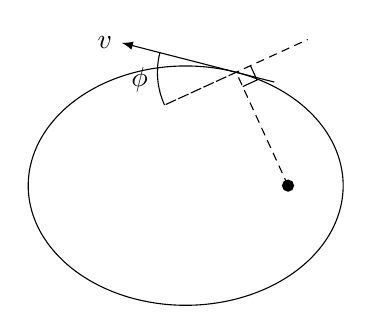
\begin{tikzpicture}[>=latex]
        \def\ecc{0.65}
        \def\SMA{2}
        \def\thta{2}
        \def\ap{\fpeval{\SMA*(1+\ecc)}}
        \def\pe{\fpeval{\SMA*(1-\ecc)}}
        \def\slr{\fpeval{\SMA*(1-\ecc^2)}}
        \def\arcRad{1}
        \def\Ra{\fpeval{\slr/(1+\ecc*cos(\thta))}}
        \def\yAB{\fpeval{sin(\thta)*\Ra}}
        \def\xB{\fpeval{(2*\SMA*\ecc)+cos(\thta)*\Ra}}
        \def\thtaA{\fpeval{pi-\thta}}
        \def\thToPt{\fpeval{(-\thtaA+atan(\yAB/\xB))/2}}

        \coordinate (pt) at ({deg(\thta)}:{\slr/(1+\ecc*cos(\thta r))}) {};
        \coordinate (o) at (\SMA-\pe,0) {};

        \draw[densely dashed] (0,0) -- (pt);

        \draw[domain=0:2*pi,samples=500, thin] plot ({deg(\x)}:{(\slr)/(1+\ecc*cos(\x r))});
        \draw[densely dashed] (pt) -- +({deg(\thta)+90}:1)-- +({deg(\thta)-90}:1);
        \draw[thin] (pt)++({deg(\thta)+180}:0.2)-- ++({deg(\thta)-90}:0.2)-- ++({deg(\thta)}:0.2);
        \draw[->] (pt) -- +({deg(\thToPt)}:0.5)--+({deg(\thToPt)-180}:1.5) node[left] {$\vv{v}$};

        \draw[] (pt)+({deg(\thta)+90}:\arcRad) arc ({deg(\thta)+90}:{deg(\thToPt)+180}:\arcRad) node[midway, left] {$\phi$};

        \filldraw[] (0,0) circle (2pt);
    \end{tikzpicture}
    \caption{An orbit with the flight path angle $\phi$ indicated}
\end{figure}

Angular momentum (Equations  \eqref{Angular Momentum Geometric Definition} and  \eqref{Angular Momentum Physical Definition}) can be used to find $\phi$.
\begin{align*}
    rv_\perp                                       & = \sqrt{a\mu(1-e^2)}                                       \\
    rv\cos(\phi)                                   & = \sqrt{a\mu(1-e^2)}                                       \\
    r\cos(\phi)\sqrt{\frac{2\mu}{r}-\frac{\mu}{a}} & = \sqrt{a\mu(1-e^2)}                                       \\
    \cos(\phi)\sqrt{2r\mu-\frac{r^2\mu}{a}}        & = \sqrt{a\mu(1-e^2)}                                       \\
    \cos(\phi)                                     & = \frac{\sqrt{a\mu(1-e^2)}}{\sqrt{2r\mu-\frac{r^2\mu}{a}}} \\
    \cos(\phi)                                     & = \sqrt{\frac{a\mu(1-e^2)}{2r\mu-\frac{r^2\mu}{a}}}        \\
    \cos(\phi)                                     & = \sqrt{\frac{a^2(1-e^2)}{2ra-r^2}}                        \\
    \cos(\phi)                                     & = \sqrt{\frac{a^2(1-e^2)}{r(2a-r)}}
\end{align*}

Note that even in hyperbolic orbits the argument of the square root is positive, so $\cos(\phi)$ is always real. $\phi$ can be found with an arccosine, keeping in mind that arccosine loses a solution. $\phi$ is positive when the satellite is getting further from the orbited body, and negative when it's getting closer. Therefore, the sign of $\phi$ is the same as the sign as $\vv{r}\cdot\vv{v}$
\begin{equation}\label{Flight Path Angle}
    \phi=\arccos{\sqrt{\frac{a^2(1-e^2)}{r(2a-r)}}}
\end{equation}


An equation has already been found relating $r$ and $\theta$, meaning this formula \textit{can} be put in terms of $\theta$. Solving for this expression, however, is left as an exercise to the reader.

\bigskip\bigskip
\subsection{True Anomaly}
Using the orbit equation (Equation  \eqref{Polar Final}), the angle $\theta$ to the periapsis can be found.
\begin{align*}
    r               & =\frac{a(1-e^2)}{1+e\cos(\theta)} \\
    1+e\cos(\theta) & =\frac{a(1-e^2)}{r}               \\
    \cos(\theta)    & =\frac{a(1-e^2)}{er}-\frac{1}{e}  \\
\end{align*}

When taking the inverse cosine, a solution will be lost. On the side of the orbit where $r$ is increasing (moving from periapsis to apoapsis) we know that $0<\theta<\pi$, while on the other side of the orbit $\pi<\theta<2\pi$. Therefore, the sign of $\theta$ (assuming $-\pi<\theta<\pi$ is taken to the the domain) is the same as the sign of $v_r$, which in turn is the same as the sign of $\vec{v}\cdot\vec{r}$.

\begin{equation}\label{True Anomoly Geometric}
    \theta=\cos^{-1}\left(\frac{a(1-e^2)-r}{er}\right)
\end{equation}

\bigskip\bigskip
\subsection{Time Since Periapsis}\label{sec:time}

Because of Kepler's second law (Section  \ref{sec:Kepler's Second Law}), there is a direct analogue between area swept out and time spent on the orbit. This allows the following relationship to be made between the time since periapsis $T_p$ and $\theta$.

\begin{align*}
    T_p(\theta) & = \frac{T}{\text{Area}}\times\text{Area swept from periapsis to }\theta                                           \\
                & = \frac{\sqrt{\frac{4\pi^2a^3}{\mu}}}{\pi{}a^2\sqrt{1-e^2}}\int_{0}^{\theta}\int_{0}^{r(\theta)}rdr d\theta       \\
                & = \frac{2\pi\sqrt{a^3}}{\pi{}a^2\sqrt{\mu(1-e^2)}}\int_{0}^{\theta}\frac{1}{2}r^2(\theta)d\theta                  \\
                & = \frac{2}{\sqrt{\mu a(1-e^2)}}\int_{0}^{\theta}\frac{1}{2}\left(\frac{a(1-e^2)}{1+e\cos(\theta)}\right)^2d\theta \\
                & = \frac{\sqrt{a^3(1-e^2)^3}}{\sqrt{\mu}}\int_{0}^{\theta}\frac{1}{(1+e\cos(\theta))^2}d\theta                     \\
\end{align*}

At this point, the transformation will be made to integrate with respect to $r$ instead of $\theta$. To do this, $\frac{d\theta}{dr}$ is needed.

\begin{align*}
    \frac{d\theta}{dr}   & = \frac{1}{dr/d\theta}                             \\
    \frac{1}{d\theta/dr} & = \frac{dr}{d\theta}                               \\
                         & =\frac{d}{d\theta}\frac{a(1-e^2)}{1+e\cos(\theta)} \\
                         & =a(1-e^2)\frac{d}{d\theta}(1+e\cos(\theta))^{-1}   \\
                         & =-a(1-e^2)(1+e\cos(\theta))^{-2}(-e\sin(\theta))   \\
                         & =\frac{ea\sin(\theta)(1-e^2)}{(1+e\cos(\theta))^2} \\
    \frac{d\theta}{dr}   & =\frac{(1+e\cos(\theta))^2}{ea\sin(\theta)(1-e^2)} \\
\end{align*}

Now, the integral can be transformed to be with respect to $r$.

\begin{align*}
    T_p & = \frac{\sqrt{a^3(1-e^2)^3}}{\sqrt{\mu}}\int_{\st{r}{pe}}^{r(\theta)}\frac{1}{\left(1+e\cos\left(\cos^{-1}\left(\frac{a(1-e^2)-r}{er}\right)\right)\right)^2}\frac{\left(1+e\cos\left(\cos^{-1}\left(\frac{a(1-e^2)-r}{er}\right)\right)\right)^2}{ea\sin\left(\cos^{-1}\left(\frac{a(1-e^2)-r}{er}\right)\right)(1-e^2)}dr \\
        & =\frac{\sqrt{a^3(1-e^2)^3}}{\sqrt{\mu}}\int_{\st{r}{pe}}^{r(\theta)}\frac{1}{\left(1+e\left(\frac{a(1-e^2)-r}{er}\right)\right)^2}\frac{\left(1+e\left(\frac{a(1-e^2)-r}{er}\right)\right)^2}{ea\sin\left(\cos^{-1}\left(\frac{a(1-e^2)-r}{er}\right)\right)(1-e^2)}dr                                                      \\
        & =\frac{\sqrt{a^3(1-e^2)^3}}{\sqrt{\mu}}\int_{\st{r}{pe}}^{r(\theta)}\frac{1}{ea\sin\left(\cos^{-1}\left(\frac{a(1-e^2)-r}{er}\right)\right)(1-e^2)}dr                                                                                                                                                                       \\
\end{align*}

The property can now be applied that $\sin(\arccos(\theta))=\sqrt{1-\theta^2}$

\begin{align*}
    T_p & =\frac{\sqrt{a^3(1-e^2)^3}}{\sqrt{\mu}}\int_{\st{r}{pe}}^{r(\theta)}\frac{1}{ea\sin\left(\cos^{-1}\left(\frac{a(1-e^2)-r}{er}\right)\right)(1-e^2)}dr                                                         \\
        & =\frac{\sqrt{a^3(1-e^2)^3}}{\sqrt{\mu}}\int_{\st{r}{pe}}^{r(\theta)}\frac{1}{ea\sqrt{1-\left(\frac{a(1-e^2)-r}{er}\right)^2}(1-e^2)}dr                                                                        \\
        & =\frac{\sqrt{a^3(1-e^2)^3}}{\sqrt{\mu}}\int_{\st{r}{pe}}^{r(\theta)}\frac{1}{ea\sqrt{1-\left(\frac{a^2(1-e^2)^2-2ar(1-e^2)+r^2}{e^2r^2}\right)}(1-e^2)}dr                                                     \\
        & =\frac{\sqrt{a^3(1-e^2)^3}}{\sqrt{\mu}}\int_{\st{r}{pe}}^{r(\theta)}\frac{1}{ea\sqrt{\frac{e^2r^2-a^2(1-e^2)^2+2ar(1-e^2)-r^2}{e^2r^2}}(1-e^2)}dr                                                             \\
        & =\frac{\sqrt{a^3(1-e^2)^3}}{\sqrt{\mu}}\int_{\st{r}{pe}}^{r(\theta)}\frac{er}{ea\sqrt{-r^2(1-e^2)-a^2(1-e^2)^2+2ar(1-e^2 )}(1-e^2)}dr                                                                         \\
        & =\frac{\sqrt{a^3(1-e^2)^3}}{\sqrt{\mu}}\int_{\st{r}{pe}}^{r(\theta)}\frac{r}{a(1-e^2)^{3/2}\sqrt{-r^2-a^2(1-e^2)+2ar}}dr                                                                                      \\
        & =\sqrt{\frac{a}{\mu}}\int_{\st{r}{pe}}^{r(\theta)}\frac{r}{\sqrt{-r^2-a^2(1-e^2)+2ar}}dr                                                                                                                      \\
        & =\sqrt{\frac{a}{\mu}}\int_{\st{r}{pe}}^{r(\theta)}\frac{r}{\sqrt{-(r-a)^2+a^2(1-(1-e^2))}}dr                                                                                                                  \\
        & =\sqrt{\frac{a}{\mu}}\int_{\st{r}{pe}}^{r(\theta)}\frac{r}{\sqrt{-(a-r)^2+a^2e^2}}dr                                                                                                                          \\
        & \phantom{=}\qquad{}\text{Substitution: }(a-r)=u_1\qquad{}du_1=-dr                                                                                                                                              \\
        & =\sqrt{\frac{a}{\mu}}\int_{a-\st{r}{pe}}^{a-r(\theta)}\frac{u_1-a}{\sqrt{-u_1^2+a^2e^2}}du_1                                                                                                                  \\
        & =\sqrt{\frac{a}{\mu}}\left(\int_{a-\st{r}{pe}}^{a-r(\theta)}\frac{u_1}{\sqrt{a^2e^2-u_1^2}}du_1-\int_{a-\st{r}{pe}}^{a-r(\theta)}\frac{a}{\sqrt{a^2e^2-u_1^2}}du_1\right)                                    \\
        & \phantom{=}\qquad{}\text{Substitution: }a^2e^2-u_1^2=u_2\qquad{}du_2=-2u_1du_1                                                                                                                                 \\
        & =\sqrt{\frac{a}{\mu}}\left(\int_{(ae)^2-(a-\st{r}{pe})^2}^{(ae)^2-(a-r(\theta))^2}\frac{-0.5}{\sqrt{u_2}}du_2-\int_{a-\st{r}{pe}}^{a-r(\theta)}\frac{a}{ae\sqrt{1-\left(\frac{u_1}{ae}\right)^2}}du_1\right) \\
        & \phantom{=}\qquad{}\text{Substitution: }\frac{u_1}{ae}=u_3\qquad{}du_3=\frac{1}{ae}du_1                                                                                                                        \\
        & =\sqrt{\frac{a}{\mu}}\left(\frac{-1}{2}\int_{(ae)^2-(a-\st{r}{pe})^2}^{(ae)^2-(a-r(\theta))^2}u_2^{-1/2}du_2+a\int_{(a-\st{r}{pe})/ae}^{(a-r(\theta))/ae}\frac{-1}{\sqrt{1-u_3^2}}du_3\right)                \\
        & =\sqrt{\frac{a}{\mu}}\left(-\Big(\sqrt{u_2}\Big)_{(ae)^2-(a-\st{r}{pe})^2}^{(ae)^2-(a-r(\theta))^2}+a\Big(\cos^{-1}(u_3)\Big)_{(a-\st{r}{pe})/ae}^{(a-r(\theta))/ae}\right)                                  \\
        & =\sqrt{\frac{a}{\mu}}\left(a\Big(\cos^{-1}(u_3)\Big)_{(a-\st{r}{pe})/ae}^{(a-r(\theta))/ae}-\Big(\sqrt{u_2}\Big)_{(ae)^2-(a-\st{r}{pe})^2}^{(ae)^2-(a-r(\theta))^2}\right)                                   \\
        & =\sqrt{\frac{a}{\mu}}\left(a\cos^{-1}\left(\frac{a-r}{ae}\right)\Big|_{\st{r}{pe}}^{r(\theta)}-\sqrt{(ae)^2-(a-r)^2}\Big|_{\st{r}{pe}}^{r(\theta)}\right)                                                    \\
        & =\sqrt{\frac{a}{\mu}}\left(a\cos^{-1}\left(\frac{a-r}{ae}\right)-\sqrt{(ae)^2-(a-r)^2}\right)_{\st{r}{pe}}^{r(\theta)}                                                                                        \\
        & =\sqrt{\frac{a}{\mu}}\left(a\cos^{-1}\left(\frac{a-r}{ae}\right)-a\sqrt{e^2-\left(1-\frac{r}{a}\right)^2}\right)_{\st{r}{pe}}^{r(\theta)}                                                                     \\
        & =\sqrt{\frac{a^3}{\mu}}\left(\cos^{-1}\left(\frac{a-r}{ae}\right)- \sqrt{e^2-\left(1-\frac{r}{a}\right)^2}\right)_{\st{r}{pe}}^{r(\theta)}                                                                    \\
\end{align*}

When the function is evaluated at $\st{r}{pe}$, the result is $0$. This means that the lower bound of the function can be removed, and the upper bound can be set as the singular argument of the function.

The time since periapsis for an orbit can be evaluated at any radius $r$ with
\begin{equation}\label{Time since periapsis}
    t_p(r)=\sqrt{\frac{a^3}{\mu}}\left(\cos^{-1}\left(\frac{a-r}{ae}\right)- \sqrt{e^2-\left(1-\frac{r}{a}\right)^2}\right)
\end{equation}

This function is only defined from the periapsis radius to the apoapsis radius, and will return a complex value for any radius outside these bounds. For hyperbolic and parabolic orbits, the function does not apply either. In a circular orbit, the argument of arccosine is $\frac{0}{0}$, so the function cannot be evaluated. This function only covers the first half of an orbit. After apoapsis, an orbit will return to every radius between the apoapsis and periapsis before once more arriving at periapsis. To find the time it takes to reach a point on this side of the orbit, simply subtract the result of this function from the period of the orbit.

\bigskip\bigskip
\subsection{Conclusion}

Throughout this section, many geometric relationships have been found describing orbits. Most importantly, it has been shown that an orbital trajectory can be described in its plane using only two parameters: the semi-major axis $a$ and the eccentricity $e$. These relationships are summarized here.

\bigskip
The angular momentum is
\[h=\sqrt{a\mu(1-e^2)}\]

\bigskip
The specific energy of an orbit is
\[\varepsilon=\frac{v^2}{2}-\frac{\mu}{r}=\frac{-\mu}{2a}\]

\bigskip
The period of an elliptic orbit is
\[P=\sqrt{\frac{4\pi^2a^3}{\mu}}\]

\bigskip
The velocity at any point in an orbit can be found with
\[v=\sqrt{\frac{2\mu}{r}-\frac{\mu}{a}}\]

Velocity for circular orbit is
\[\st{v}{circ}=\sqrt{\frac{\mu}{r}}\]

Escape velocity at any altitude is
\[\st{v}{escape}=\sqrt{\frac{2\mu}{r}}=\st{v}{circ}\sqrt{2}\]

\bigskip
While the flight path angle can be found as
\[\phi=\arccos\left(\sqrt{\frac{a^2(1-e^2)}{r(2a-r)}}\right)\]

\bigskip
The true anomaly can be found in an orbit with
\[\theta=\arccos\left(\frac{a(1-e^2)-r}{er}\right)\]

\bigskip
The time since periapsis in any noncircular elliptic orbit can be found with
\[t_p(r)=\sqrt{\frac{a^3}{\mu}}\left(\cos^{-1}\left(\frac{a-r}{ae}\right)- \sqrt{e^2-\left(1-\frac{r}{a}\right)^2}\right)\]


\end{document}